%%%%%%%%%%%%%%%%%%%%%%%%%%%%%%%%%%%%%%%%%
% Original author:
% Linux and Unix Users Group at Virginia Tech Wiki
% (https://vtluug.org/wiki/Example_LaTeX_chem_lab_report)
% Modified by: Hector F. Jimenez S, for the Digital Electronics Laboratory.
% License:
% CC BY-NC-SA 3.0 
%%%%%%%%%%%%%%%%%%%%%%%%%%%%%%%%%%%%%%%%%
%----------------------------------------
%	PACKAGES AND DOCUMENT CONFIGURATIONS
%---------------------------------------

\documentclass[paper=a4, fontsize=12pt]{article} 		% A4 paper and 11pt font size
\usepackage[T1]{fontenc} 								% Use 8-bit encoding that has 256 glyphs
%\usepackage{fourier}		 							% Use the Adobe Utopia font for the document 
\usepackage[spanish,english]{babel}						% Spanish Language, templates uses some sections in english.
\selectlanguage{spanish}								% main language.
\PassOptionsToPackage{spanish}{babel}
%\renewcommand{\figurename}{Figura}						% Force rename of figure.
%\renewcommand{\figurename}{Fig.}
\usepackage[figurename=Fig.]{caption}
\usepackage[utf8]{inputenc}								% tildes for spanish language.
\usepackage{amsmath,amsfonts,amsthm} 					% Math packages.
\usepackage{minted}										% For syntax highlighting.
\usepackage{float}										% Image will be in the same place as you want.!!! x-/
\usepackage{sectsty} 									% Allows customizing section commands
\allsectionsfont{\centering \normalfont\scshape}	   	% Make all sections centered, the default font and small caps
\usepackage{hyperref}
\hypersetup{											%Setups the false color and borders.
    colorlinks=false,
    pdfborder={0 0 0},
}
\newcommand\fnurl[2]{%									% set a simple and quick footnote command and include url.
\href{#2}{#1}\footnote{\url{#2}}%	
}
\usepackage{graphicx}									% Import easyly images.
\graphicspath{ {./images/} }							% Where to look for the images.
\DeclareGraphicsExtensions{.pdf,.png,.jpg}				% Graphics Extension to be used
\usepackage[notes,backend=biber]{biblatex-chicago}		% Bibliography and references.
\bibliography{biblio}									% bibliography filename.
\usepackage{fancyhdr} 									% Custom headers and footers
\pagestyle{fancyplain} 									% Makes all pages in the document conform to the custom headers and footers
\fancyhead{} 											% No page header
\fancyfoot[L]{} 										% Empty left footer
\fancyfoot[C]{} 										% Empty center footer
\fancyfoot[R]{\thepage} 								% Page numbering for right footer
\renewcommand{\headrulewidth}{0pt} 						% Remove header underlines
\renewcommand{\footrulewidth}{0pt} 						% Remove footer underlines
\setlength{\headheight}{13.6pt} 					    % Customize the height of the header
\numberwithin{equation}{section}						% Number equations within sections (i.e. 1.1, 1.2, 2.1, 2.2 instead of 1, 2, 3, 4)
%\numberwithin{figure}{section} 						% Number figures within sections (i.e. 1.1, 1.2, 2.1, 2.2 instead of 1, 2)
\numberwithin{table}{section} 							% Number tables within sections (i.e. 1.1, 1.2, 2.1, 2.2 instead of 1, 2, 3, 4)
\setlength\parindent{0pt} 								% Removes all indentation from paragraphs

%\newcommand{\horrule}[1]{\rule{\linewidth}{#1}} 		% Create horizontal rule command with 1 argument of height
%%%%%%%%%%%%%%%%%%%%
%Title Section
%%%%%%%%%%%%%%%%%%%%%
\title{Desarrollo de un Controlador de Tráfico\\ 
Usando FPGA's \\
Laboratorio de Electrónica Digital\\Módulo: 1} 			% Title
%\horrule{0.5pt} \\[0.4cm] 								% Thin top horizontal rule	Title rule
%\huge Assignment Title \\ 								% The assignment title
%\horrule{2pt} \\[0.5cm] 								% Thick bottom horizontal rule
\author{												% Authors begin.
Héctor F. \textsc{Jiménez Saldarriaga}\\
\texttt{hfjimenez@utp.edu.co} \\
\texttt{PGP KEY ID: 0xB05AD7B8}
\and
Steffany \textsc{Lopez Segura}\\
\texttt{steffany@utp.edu.co}
} 												       % End of  Author name
\date{}    						                       % Date for the report, this will hide the \today.

\begin{document}
\maketitle                      			           % Insert the title, author and date
\begin{center}
\begin{tabular}{l r}								   % two column to
Fecha de Entrega: & Febrero 24, 2016 \\				   % Ramiro's Details.
Profesor: & Ing.Msc(c) Ramiro Andres Barrios Valencia
\end{tabular}
\end{center}
%%%%%%%%%%%	
% Let's start the document.
%%%%%%%%%%%	
\section{Objectivos}
\begin{itemize}
  \item Fortalecer y poner en práctica la teoría de circuitos combinacionales.
  \item Fortalecer el desarrollo de sistemas digitales, utilizando el lenguaje \emph{VHDL} y el entorno de desarrollo Xilinx ISE.
\end{itemize}

%%%%%%%%%%%	
% Theory Marc! 
%%%%%%%%%%%	
\section{Marco Teórico}
\label{sec:problemamecanico}
sometext \ref{fig:debounce}.\\
\begin{figure}[H]
  \centering
     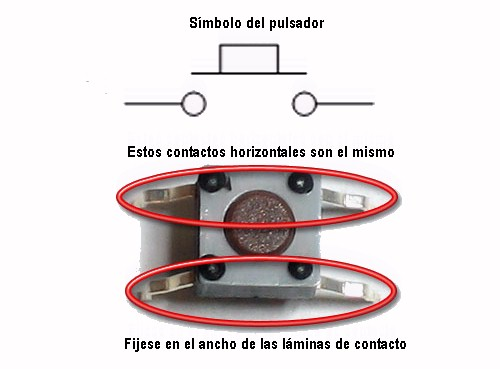
\includegraphics[width=0.5\textwidth]{pulsador}
  \caption{Pulsador Común, Composición.}
      \label{fig:pulsador}
\end{figure}

\label{sec:pulsador} 
En algunos casos esta acción puede producir una chispa debido a la corriente que atraviesa los contactos, disminuyendo el tiempo útil de los contactos eléctricos. La chispa se produce siempre al separar los contactos 
\begin{figure}[H]
  \centering
     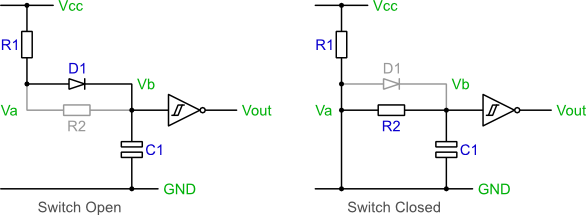
\includegraphics[width=0.7\textwidth]{debounceCircuit2}
  \caption{Solución utilizando un simple arreglo electrónico. Pulsadores con resistencias de Pull Ups.}
      \label{fig:hardwc}
\end{figure}
\section{Arquitectura de la Placa \emph{NEXYS 2}}
La tarjeta de entrenamiento \emph{NEXYS 2} 
\begin{description}
  \item[Connectores] \hfill \\
  	\begin{itemize}
		\item Puerto USB2.0
	    \item Puerto VGA
    \end{itemize}

Algunas de las que más nos llamaron la atención son:\\
  \item[Caracteristicas] \hfill \\
    	\begin{itemize}
			\item Xilinx Spartan-3E FPGA 500K
  			\item Incluye  8 leds, cuatro display siete segmentos, cuatro pulsadores, 8 switches.\ldots
      \end{itemize}
\end{description}
\begin{figure}[H]
  \centering
     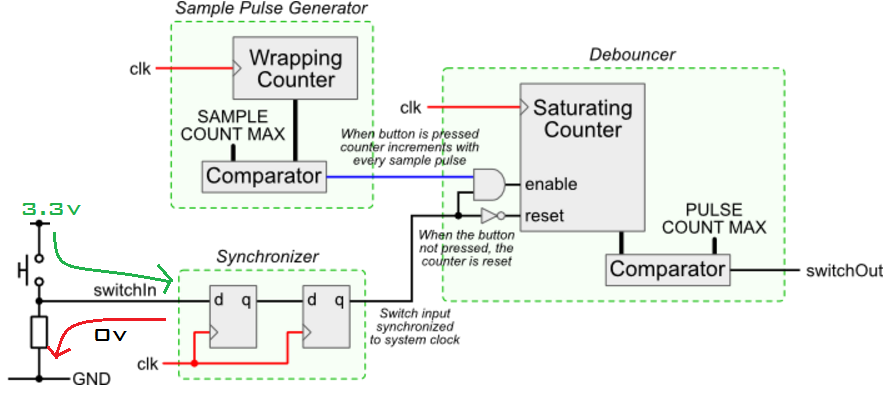
\includegraphics[width=1\textwidth]{implementacion}
  \caption{Desarrollo a implementar. Tiempo para presionar el pulsador mínimo de 33mS}
  \label{fig:eliteimplemetacion}
\end{figure}
\section{Explicación Código VHDL}
Descripción del Pseudo código para el módulo anti rebote:
\begin{minted}{vhdl}
 1 Setup a counter variable, initialise to zero.
 2 Setup a regular sampling event, perhaps using a timer. Use a period of about 1ms.
 3 On a sample event:
 4   if switch signal is high then
 5     Reset the counter varaible to zero
 6     Set internal switch state to released
 7   else
 8     Increment the counter variable to a maximum of 10
 9   end if
10   if counter=10 then
11     Set internal switch state to pressed
12   end if
\end{minted}
Código de Ejemplo de Anti-Rebote.
%\inputminted{vhdl}{./Code/debounce.vhd}
\section{Prácticas Experimentales}
Fotos de la Simulación y Conclusiones.
\section{Anexos}
Se adjunta el código en un archivo comprimido de nombre \textsc{module1.zip}, los demás archivos son adicionales que resuelven la misma implementación.
\textit{Nota}: Las referencias utilizadas se encuentran en los pies de página. Si requiere de manera detallada estas contacte con \emph{hfjimenez@utp.edu.co}
\end{document}